\documentclass[11pt,a4paper]{article}
\usepackage[utf8]{inputenc}
\usepackage[a4paper,margin=2.5cm]{geometry}
\usepackage{amsmath,amssymb,amsthm,mathtools}
\usepackage{booktabs,longtable,array}
\usepackage{enumitem}
\usepackage{tikz}
\usetikzlibrary{arrows.meta,calc}
\usepackage[font=small,labelfont=bf]{caption}
\usepackage{fancyhdr}
\usepackage{microtype}
\usepackage[colorlinks=true,linkcolor=blue!45!black,citecolor=blue!45!black,urlcolor=blue!45!black,pdfauthor={Aryan Kumar Singh},pdftitle={The Top-Down Cascade Method for Stick-Slip Analysis in Stacked Friction Systems, Version 2}]{hyperref}

\newcolumntype{R}[1]{>{\raggedleft\arraybackslash}p{#1}}
\newtheorem{proposition}{Proposition}
\newtheorem{definition}{Definition}

\newcommand{\fs}{f^{\mathrm{s}}}
\newcommand{\fkin}{f^{\mathrm{k}}}
\newcommand{\mus}{\mu^{\mathrm{s}}}
\newcommand{\muk}{\mu^{\mathrm{k}}}
\DeclareMathOperator{\sgn}{sgn}
\newcommand{\Freq}{F_{\mathrm{req}}}

\setlength{\headheight}{14pt}
\pagestyle{fancy}
\fancyhf{}
\fancyhead[L]{\small Top-Down Cascade Method, Version 2}
\fancyhead[R]{\small A.\,K.\ Singh}
\fancyfoot[C]{\small\thepage}
\renewcommand{\headrulewidth}{0.3pt}
\setlist[itemize]{itemsep=2pt,topsep=4pt}
\setlist[enumerate]{itemsep=2pt,topsep=4pt}

\begin{document}

\title{The Top-Down Cascade Method for Stick--Slip Analysis\\
in Stacked Friction Systems\\[6pt]
\large Version 2: Separate Static and Kinetic Friction\\
(the SLIP-SPLIT-CALCULATE Algorithm)}
\author{Aryan Kumar Singh\\[2pt]
\normalsize High school student, India\\[2pt]
\normalsize\texttt{skosunilsingh@gmail.com}}
\date{October 30, 2026}
\maketitle
\thispagestyle{plain}

\begin{abstract}
\noindent The Top-Down Cascade Method finds the instantaneous acceleration of every block in a vertical stack of rigid blocks joined by dry friction, with an independent horizontal force on each block. Version 1 assumed that the coefficient of static friction equals the coefficient of kinetic friction at every interface. This paper presents version 2, which allows a different static coefficient and a different kinetic coefficient at every interface. Two rules carry the original procedure over to that case: every test of whether an interface holds uses its static limit, and every force exerted by an interface that has slipped is its kinetic friction. A fifth phase, the re-join, is added. It corrects the interfaces whose assumed sliding direction is contradicted by the accelerations that the first four phases produce. The paper gives the procedure, three small examples, the thirty-block system of version 1 solved by hand with kinetic friction at 80\% of the static value, a proof that the answer is unique when the two coefficients are equal, and an example in which they are not. The method was compared with exhaustive enumeration on 34\,000 random stacks of two to eight blocks, and with an independent minimisation on 100 stacks of 20 to 119 blocks. With equal coefficients it gave the exact answer in every test. With a larger static coefficient, Coulomb's law can allow more than one self-consistent answer. The method returns one of them by a fixed rule, and a time-stepping simulation shows that the behaviour of a real stack can depend on how fast friction falls from its static to its kinetic value.
\end{abstract}

\tableofcontents

\section{Introduction}

A stack of rigid blocks held together by dry friction is a standard problem in mechanics. A horizontal force on one block may move that block alone, may move several blocks together, or may move nothing, depending on whether each friction interface can carry the force that reaches it. Crates on a pallet, plates in a friction clutch and layers of ground under a sideways load are examples.

Version 1 of the Top-Down Cascade Method~\cite{singh1} finds the accelerations of all blocks in one pass from the top of the stack to the bottom. At each interface it compares a running drive force with a friction limit. A block or group that slips passes the friction of its interface down to the next block. A group that sticks together is checked from the inside and is split wherever its own interfaces cannot supply the force that a shared acceleration requires. Version 1 assumed that the coefficient of static friction equals the coefficient of kinetic friction at every interface. One number, $f_i$, then served both as the largest force that interface $i$ can hold and as the force it exerts when it slips.

That assumption often does not hold. For most pairs of surfaces the static coefficient is larger than the kinetic coefficient, and problems usually give both. A block at rest stays at rest until the force on it exceeds $\mus N$; once it slips, the friction is $\muk N$. In a stack this has two effects. The friction that a slipping interface passes to the block below is smaller, so the next interface may hold where, with equal coefficients, it would have slipped. And the interfaces inside a sliding group were at rest when the motion began, so they are checked against their static limits, while the force they exert after they fail is kinetic.

This paper presents version 2, which handles both coefficients. Two rules extend the earlier procedure. Every test of whether an interface holds uses its static limit. Every force exerted by an interface that slips is its kinetic friction. One phase is added, the re-join (Phase 5). It is needed because the first four phases fix the sliding direction at each interface from the sign of a force, and the accelerations that result sometimes contradict that direction (Examples 2 and 3, Section~\ref{sec:examples}). In the tests of Section~\ref{sec:tests}, the first four phases alone gave an admissible result for between 54.0\% and 87.8\% of random small stacks with equal coefficients, and for none of the 200 random stacks of 500 blocks. Phase 5 corrects those interfaces and does nothing when there is nothing to correct.

The limits of the method are stated where they arise. When the static coefficient is larger than the kinetic coefficient, Coulomb's law alone can allow more than one self-consistent set of accelerations (Section~\ref{sec:several}). The method returns one of them by a fixed rule. It does not claim that every real stack behaves in that way.

Section~\ref{sec:notation} gives the notation and Section~\ref{sec:method} the procedure. Section~\ref{sec:examples} works three small examples and the thirty-block system of version 1. Section~\ref{sec:guarantees} states what the procedure guarantees and what it does not. Section~\ref{sec:tests} describes the tests. Section~\ref{sec:discussion} discusses the scope. Appendix~\ref{app:derivation} gives the full hand solution of the thirty-block system, and Appendix~\ref{app:random} describes the random stacks used in the tests.

\section{Problem Definition and Notation}\label{sec:notation}

Consider $n$ rigid blocks arranged in a vertical column and labelled $1$ (top) to $n$ (bottom); block $n$ rests on a fixed floor. Block $i$ has mass $m_i$ and may carry an external horizontal force $F_i$, applied directly to that block and independent of the force on any other block. A single global horizontal axis is fixed for the entire problem, with rightward taken as positive; every force, velocity and acceleration in this paper is a signed scalar measured along that axis. All blocks are at rest at the start, and the quantity sought is the acceleration of each block at the first instant of motion.

Blocks $i$ and $i+1$ meet at a horizontal interface, denoted interface $i$, for $i=1,\dots,n-1$; interface $n$ is the contact between block $n$ and the fixed floor. Every external force is horizontal, so the normal force across interface $i$ is the weight of blocks $1$ to $i$, whether or not anything moves:
\[
N_i=g\,M_i,\qquad M_i=m_1+m_2+\dots+m_i .
\]
Interface $i$ has a coefficient of static friction $\mus_i$ and a coefficient of kinetic friction $\muk_i$, with $0\le\muk_i\le\mus_i$. Two forces follow from them:
\[
\fs_i=\mus_i N_i,\qquad \fkin_i=\muk_i N_i .
\]
The static limit $\fs_i$ is the largest shear force that interface $i$ can supply while it sticks. The kinetic friction $\fkin_i$ is the magnitude of the force it supplies once it slips. In version 1 the two were equal and were written $f_i$. Here $\fkin_i=\fs_i$ is the special case $\muk_i=\mus_i$.

Let $R_i$ be the friction force that interface $i$ exerts on block $i$, which is the block above it. By Newton's third law the same interface exerts $-R_i$ on block $i+1$. Newton's second law for block $i$ is
\begin{equation}\tag{N}\label{eq:N}
m_i a_i=F_i-R_{i-1}+R_i,\qquad i=1,\dots,n,
\end{equation}
with $R_0=0$ (nothing lies above block 1) and $a_{n+1}=0$ (the floor does not move). Let $\rho_i=a_i-a_{i+1}$ be the relative acceleration of the two blocks at interface $i$. At the first instant all velocities are zero, and the friction law is
\begin{align}
\tag{F1}\label{eq:F1}
\rho_i=0&\;\Longrightarrow\;|R_i|\le \fs_i &&\text{(the interface sticks),}\\
\tag{F2}\label{eq:F2}
\rho_i\ne0&\;\Longrightarrow\;R_i=-\sgn(\rho_i)\,\fkin_i &&\text{(the interface slips).}
\end{align}
Friction opposes the relative acceleration, and it has the kinetic value as soon as the interface slips. A set of accelerations $a_i$ and forces $R_i$ that satisfies \eqref{eq:N} at every block and \eqref{eq:F1} or \eqref{eq:F2} at every interface is called an \emph{admissible state}. Every result in this paper is judged by whether it is admissible.

Figure~\ref{fig:blocks} shows three consecutive blocks from the interior of a stack. The input data of the thirty-block system used in Section~\ref{sec:examples} are in Table~\ref{tab:input30}.

\begin{figure}[ht]
\centering
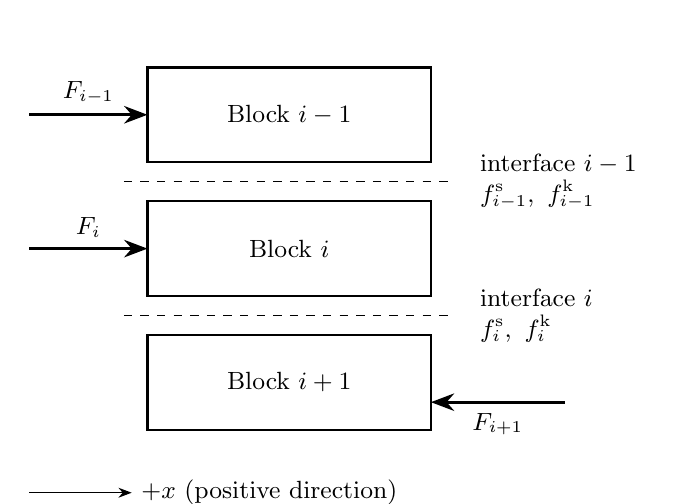
\begin{tikzpicture}[>=Stealth,font=\small]
  \draw[thick] (0,3.6) rectangle (3.6,4.8); \node at (1.8,4.2) {Block $i-1$};
  \draw[thick] (0,1.9) rectangle (3.6,3.1); \node at (1.8,2.5) {Block $i$};
  \draw[thick] (0,0.2) rectangle (3.6,1.4); \node at (1.8,0.8) {Block $i+1$};
  \draw[dashed] (-0.3,3.35) -- (3.9,3.35);
  \draw[dashed] (-0.3,1.65) -- (3.9,1.65);
  \node[anchor=west,align=left] at (4.1,3.35) {interface $i-1$\\$\fs_{i-1},\ \fkin_{i-1}$};
  \node[anchor=west,align=left] at (4.1,1.65) {interface $i$\\$\fs_{i},\ \fkin_{i}$};
  \draw[->,very thick] (-1.5,4.2) -- (0,4.2) node[midway,above] {$F_{i-1}$};
  \draw[->,very thick] (-1.5,2.5) -- (0,2.5) node[midway,above] {$F_{i}$};
  \draw[->,very thick] (5.3,0.55) -- (3.6,0.55) node[midway,below] {$F_{i+1}$};
  \draw[->] (-1.5,-0.6) -- (-0.2,-0.6) node[right] {$+x$ (positive direction)};
\end{tikzpicture}
\caption{General arrangement of three consecutive blocks. Each block carries its own external force along the single global axis ($F_{i+1}$ is drawn as a negative force). Each interface below a block has a static limit $\fs$ and a kinetic friction $\fkin$, with $\fkin\le\fs$.}\label{fig:blocks}
\end{figure}

\section{The Top-Down Cascade Method, Version 2}\label{sec:method}

The method proceeds in five phases. Phase 1 is carried out once, at the outset. Phase 2 is repeated as each new block is reached while scanning down the stack. Phase 3 is the rule by which a result already found for one block or group is passed to the block beneath it. Phase 4 is a fail-safe check applied whenever blocks have been provisionally grouped by sticking. Phase 5 is a final check of the sliding directions, with repairs.

Version 2 differs from version 1 in three places, which together make the rule \textbf{test with $\fs$, push with $\fkin$}:
\begin{enumerate}
\item Every question of the form ``does this interface hold?'' (Phase 2, and the internal checks of Phase 4) is put to the static limit $\fs$.
\item Every force that an interface exerts after it has slipped (Phase 3, the bottom of a sliding group, and the two sides of a fracture) is the kinetic friction $\fkin$.
\item Phase 5 is new.
\end{enumerate}

\subsection{Phase 1: System Initialization}

Fix the global sign convention once, before any block is examined. Compute the static limit $\fs_i=\mus_i g M_i$ and the kinetic friction $\fkin_i=\muk_i g M_i$ at every interface, with $\fkin_i\le\fs_i$. If a problem gives only one coefficient for an interface, take $\fkin_i=\fs_i$, which is version 1. All forces used afterward are signed quantities measured along this single axis, and the axis is not changed for the remainder of the calculation.

\subsection{Phase 2: Boundary Evaluation (Top-Down Progression)}

Working down from the top of the stack, maintain a candidate group that begins as a single block and may grow as further blocks are added to it. Suppose the group currently spans blocks $p$ through $q$ (initially $p=q=1$), and let $C$ denote the force transmitted into this group from whatever lies immediately above block $p$ ($C=0$ if $p=1$). The drive on the group is
\begin{equation}\label{eq:D}
D=C+\sum_{i=p}^{q}F_i .
\end{equation}
Compare $|D|$ with $\fs_q$, the static limit of the interface directly beneath the group.
\begin{itemize}
\item If $|D|\le \fs_q$: interface $q$ holds. Block $q+1$ is added to the group ($q\to q+1$), and the comparison in Equation~\eqref{eq:D} is repeated against the new static limit. If $q=n$, the group has reached the floor and holds against it. The whole group is then at rest ($a=0$), and the force that each of its interfaces supplies is the balance of everything above that interface.
\item If $|D|>\fs_q$: interface $q$ yields. The group slides in the direction of $D$, and the interface exerts on it the kinetic friction $\fkin_q$, opposite to $D$. If the group is a single block ($p=q$), its acceleration is found immediately (Equation~\eqref{eq:single} below). If the group contains more than one block, its members cannot be assigned this acceleration until it has been checked that every interface between them can actually sustain it; that check is Phase 4.
\end{itemize}
The static limit is used in this test because every interface starts at rest. The kinetic friction plays no part in it.

\subsection{Phase 3: Load Transmission (The Cascade)}

Once a block or group's acceleration has been finalized, the interface immediately beneath it is, by construction, the one that was found to yield. That interface exerts a kinetic friction force of magnitude $\fkin_q$, directed the same way the group above it is sliding, onto the block immediately below. This transmitted force becomes the new carried-in force $C$ for the next, still-unresolved part of the stack, and Phase 2 resumes there.

For a single block that yields on its own (a group of size one), the acceleration follows directly:
\begin{equation}\label{eq:single}
a=\frac{D-\fkin\,\sgn(D)}{m},
\end{equation}
where $m$ is the block's mass, $\fkin$ is the kinetic friction of the interface directly beneath it, and $\sgn(D)=+1$ if $D>0$ and $-1$ if $D<0$. The quantity $\fkin\sgn(D)$ is the value carried forward to the next block under this phase.

In version 1 the carried force was $f_q\sgn(D)$. It is now $\fkin_q\sgn(D)$, which is smaller or equal. This is the first way in which the kinetic coefficient changes a result: the next block receives less.

\subsection{Phase 4: Internal Shear Verification (The Fail-Safe)}

Suppose Phase 2 has extended a candidate group across blocks $p$ through $q$ before finding that interface $q$ yields under drive $D$. Because the group has more than one member, its acceleration cannot be accepted until every interface between blocks $p$ and $q$ has been shown able to carry the force that a shared acceleration would require of it.

Let $T$ be the force on block $p$ from above and $B$ the force on block $q$ from below. For a group just formed by Phase 2, $T=C$ and $B=-\fkin_q\sgn(D)$, so that $T+\sum F_i=D$. The acceleration the whole group would have if it stayed rigid is
\begin{equation}\label{eq:a0}
a^{(0)}=\frac{T+\sum_{i=p}^{q}F_i+B}{\sum_{i=p}^{q}m_i}.
\end{equation}
For a group just formed by Phase 2 this is $(D-\fkin_q\sgn D)/\sum m_i$.

Then, starting at the interface immediately above the one that yielded (interface $q-1$) and working upward, each internal interface $j$ ($j=q-1,q-2,\dots,p$) is checked in turn. The force interface $j$ would need to supply, if blocks $p$ through $j$ are to share the acceleration $a^{(0)}$, is
\begin{equation}\label{eq:Freq}
\Freq(j)=\Bigl(\sum_{i=p}^{j}m_i\Bigr)a^{(0)}-\Bigl(T+\sum_{i=p}^{j}F_i\Bigr).
\end{equation}
If $|\Freq(j)|\le \fs_j$, interface $j$ holds under this assumption, and the check continues at $j-1$. The first interface $j^{*}$, moving upward from $q-1$, at which $|\Freq(j)|$ exceeds $\fs_j$ is where the group actually fractures. From that moment the interface slips, so it exerts its kinetic friction: the force $\fkin_{j^*}\sgn\Freq(j^*)$ on the upper part, from below, and the opposite force on the lower part, from above. Blocks $p$ through $j^{*}$ form the upper fragment, with top force $T$ and bottom force $\fkin_{j^*}\sgn\Freq(j^*)$. Blocks $j^{*}+1$ through $q$ form the lower fragment, with top force $-\fkin_{j^*}\sgn\Freq(j^*)$ and bottom force $B$. A fragment of one block has the acceleration $(T+F+B)/m$, which is Equation~\eqref{eq:single}. A fragment of more than one block is resubmitted to Phase 4, with $a^{(0)}$ recomputed from Equation~\eqref{eq:a0} for the smaller group. If no interface fails during the scan, the entire group moves together at $a^{(0)}$, and this is its final acceleration.

Version 1 wrote the force at the fracture as $f_{j^*}\sgn(a^{(0)})$. For a group formed by Phase 2 the two signs agree: Phase 2 has shown $|C+\sum_{i=p}^{j}F_i|\le \fs_j$ at every interior interface, and $|\Freq(j)|>\fs_j$ can then only happen when $\Freq(j)$ has the sign of $a^{(0)}$. For the fragments of later fractures the two signs can differ, and the sign of $\Freq$ is the one to use.

Because a fracture always shortens the group under consideration, and Phase 4 is reapplied to each fragment it produces, the process terminates after at most $q-p$ fractures, each one resolved by Equations~\eqref{eq:a0} and~\eqref{eq:Freq}.

\subsection{Phase 5: Re-join}\label{sec:phase5}

Phases 2 to 4 fix the sliding direction of an interface from the sign of a force: the sign of the drive $D$ when the interface yields, and the sign of $\Freq$ when it fractures. This is an assumption. When the block below an interface is pulled harder than the group above it, the accelerations that result can contradict the assumed direction. The lower block then ends up moving ahead of the upper one, while the friction that was used is the friction that acts when the upper block moves ahead. Examples 2 and 3 in Section~\ref{sec:examples} show this. Phase 5 finds such interfaces and corrects them.

\paragraph{Slip pattern.} A state of the stack is described by a pattern $\sigma=(\sigma_1,\dots,\sigma_n)$. Here $\sigma_i=0$ means that interface $i$ sticks. The value $\sigma_i=+1$ or $\sigma_i=-1$ means that interface $i$ slips and that $a_i-a_{i+1}$ is positive or negative; the interface then exerts $-\sigma_i\fkin_i$ on block $i$. Phases 2 to 4 produce a pattern: $\sigma_q=\sgn D$ at an interface that yields in Phase 2, $\sigma_{j^*}=-\sgn\Freq(j^*)$ at an interface that fractures in Phase 4, and $\sigma_i=0$ at every other interface.

\paragraph{Solving a pattern.} The sticking interfaces join the blocks into groups of consecutive blocks that move rigidly. For a group of blocks $p$ to $q$, the interface above exerts $T=\fkin_{p-1}\sigma_{p-1}$ on block $p$ ($T=0$ if $p=1$). If interface $q$ slips, it exerts $B=-\fkin_q\sigma_q$ on block $q$, and the group has the acceleration of Equation~\eqref{eq:a0}. If $q=n$ and interface $n$ sticks, the group rests on the floor: $a=0$ and $B=-(T+\sum F_i)$. The force that a sticking interface $j$ inside a group must supply is Equation~\eqref{eq:Freq} with the acceleration of the group in place of $a^{(0)}$.

\paragraph{Conditions.} The pattern is admissible when both of the following hold.
\begin{enumerate}[label=(\roman*)]
\item Every sticking interface $j$ supplies no more than its static limit: $|\Freq(j)|\le \fs_j$. For a group resting on the floor, the force supplied by the floor is $|B|\le \fs_n$.
\item Every slipping interface $j$ has the relative acceleration that was assumed: $\sigma_j(a_j-a_{j+1})>0$. The kinetic friction then opposes the relative acceleration.
\end{enumerate}

\paragraph{Repair steps.} Start from the pattern of Phases 2 to 4 and repeat the following.
\begin{enumerate}[label=(\alph*)]
\item If some slipping interface violates (ii), take the one for which $\sigma_j(a_j-a_{j+1})$ is the most negative and set $\sigma_j=0$. The two groups beside it re-join.
\item Otherwise, if some sticking interface violates (i), take the one with the largest ratio $|\Freq(j)|/\fs_j$ and set $\sigma_j=-\sgn\Freq(j)$. The interface slips, in the direction that the force it failed to supply demands.
\item If neither applies, stop.
\end{enumerate}
After each change the pattern is solved again. If Phases 2 to 4 already give an admissible pattern, neither (a) nor (b) applies and Phase 5 changes nothing.

Step (b) is where the static limit enters Phase 5: an interface starts to slip only when the force it has to supply exceeds $\fs_j$. The order in which overloaded interfaces are released in step (b) matters only when $\fkin<\fs$. For equal coefficients the admissible state is unique (Section~\ref{sec:equal}), so every order that ends in an admissible pattern gives the same result. The largest-ratio rule was compared with three other rules (the overloaded interface nearest the top, the one nearest the floor, and the one with the largest excess force weighted by $1/m_{\text{above}}+1/m_{\text{below}}$). All four rules reached an admissible state in all 6\,271 stacks of the comparison in which Phases 2 to 4 had failed. For $\fkin<\fs$, the largest-ratio rule returned the admissible state with the fewest interfaces differing from the pattern of Phases 2 to 4 in 5\,365 of 5\,507 stacks (97.4\%).

The repair is not proved to stop. In every test of Section~\ref{sec:tests} it stopped. A program should still limit the number of steps; the program of Section~\ref{sec:remarks} stops after $50n+50$ steps and reports that its check failed.

\subsection{Summary of the Procedure}

\begin{enumerate}
\item Fix the sign convention and compute $\fs_i$ and $\fkin_i$ for every interface (Phase 1).
\item Starting at block 1 with $C=0$, extend a candidate group one block at a time, accumulating the drive $D$ of Equation~\eqref{eq:D}, until $|D|>\fs_q$ (Phase 2).
\item If the group is a single block, find its acceleration from Equation~\eqref{eq:single} and go to step 5.
\item If the group has more than one block, compute $a^{(0)}$ from Equation~\eqref{eq:a0} and scan the internal interfaces upward from the one that just yielded, using Equation~\eqref{eq:Freq}. Split at the first interface with $|\Freq|>\fs$, give the two fragments the kinetic friction $\fkin$ of that interface with opposite signs, and resolve each fragment in the same way (Phase 4).
\item Transmit the kinetic friction $\fkin_q\sgn D$ of the interface that yielded to the next block down as the new carried-in force $C$, and return to step 2 for the remainder of the stack (Phase 3). A group that still holds when it reaches the floor is at rest.
\item When every block has an acceleration, solve the resulting pattern and check conditions (i) and (ii). Apply the repair steps of Phase 5 until none is left.
\end{enumerate}

\subsection{Remarks}\label{sec:remarks}

\paragraph{Equal coefficients.} If $\fkin_i=\fs_i$ at every interface, Phases 1 to 4 are the procedure of version 1 with $f_i=\fs_i=\fkin_i$. The program described below reproduced Table~2 of version 1 for the thirty-block system to the two decimals printed there.

\paragraph{Cost.} With prefix sums of the masses and forces, the mass or force sum of any range of blocks is available in constant time. Phases 2 to 4 then cost one pass down the stack plus the scans of Phase 4, each of which is at most as long as the group it examines. Each step of Phase 5 costs one pass over the stack, to solve the pattern and to find the next change. For random stacks of 500 blocks the mean number of steps was between 27.4 and 46.5 (Table~\ref{tab:large}).

\paragraph{Program.} A program that carries out the method is the single HTML file \texttt{slip\_\allowbreak split\_\allowbreak calculate\_\allowbreak runner\_\allowbreak v2.html}. It runs in a web browser and does not send data anywhere. Its Standard section takes one friction number per block and runs Phases 1 to 4 as in version 1. Its Advanced section takes the mass, external force, $\mus$ and $\muk$ of every block and a value of $g$, and runs Phases 1 to 5. Both sections can show a step-by-step log, the physical check of Section~\ref{sec:check}, and a moving picture of the result. The log in Appendix~\ref{app:derivation} was produced by the program.

\section{Worked Examples}\label{sec:examples}

Three small examples show the rules one at a time, and the thirty-block system of version 1 shows them together. Throughout, $g=10\,\mathrm{m/s^2}$.

\subsection{Example 1: Three Blocks, Static Limit and Kinetic Friction}\label{sec:ex1}

Three blocks, from the top, have masses $2$, $3$ and $5\,\mathrm{kg}$. The only external force is $F_2=+60\,\mathrm{N}$ on the middle block. The coefficients are $\mus=(0.5,\ 0.4,\ 0.3)$ and $\muk=(0.4,\ 0.3,\ 0.1)$.

\paragraph{Phase 1.} The normal forces are $N=(20,\ 50,\ 100)\,\mathrm{N}$. Hence $\fs=(10,\ 20,\ 30)\,\mathrm{N}$ and $\fkin=(8,\ 15,\ 10)\,\mathrm{N}$.

\paragraph{Phase 2.} Block 1: $C=0$ and $D=0$, so $|D|\le \fs_1$ and interface 1 holds; block 2 joins the group. Block 2: $D=0+60=60\,\mathrm{N}$ and $|D|>\fs_2=20\,\mathrm{N}$, so interface 2 yields. The group (1--2) slides to the right, and interface 2 exerts $\fkin_2=15\,\mathrm{N}$ on it, to the left.

\paragraph{Phase 4.} By Equation~\eqref{eq:a0}, $a^{(0)}=(60-15)/5=9.00\,\mathrm{m/s^2}$. For interface 1, $\Freq(1)=2(9.00)-0=18.00\,\mathrm{N}$, which is larger than $\fs_1=10\,\mathrm{N}$, so the group fractures there. Interface 1 now slips and exerts $\fkin_1=8\,\mathrm{N}$: block 1 receives $+8\,\mathrm{N}$ from below and block 2 receives $-8\,\mathrm{N}$ from above. Then
\[
a_1=\frac{8}{2}=4.00\,\mathrm{m/s^2},\qquad a_2=\frac{-8+60-15}{3}=12.33\,\mathrm{m/s^2}.
\]

\paragraph{Phases 3 and 2 again.} Interface 2 transmits $+15\,\mathrm{N}$ to block 3. For block 3, $D=15\,\mathrm{N}$ and $\fs_3=30\,\mathrm{N}$, so interface 3 holds. Block 3 has reached the floor, so it is at rest: $a_3=0$, and the floor supplies $-15\,\mathrm{N}$.

\paragraph{Phase 5.} At interface 1, $\rho_1=4.00-12.33<0$ and the interface exerts $+8\,\mathrm{N}$ on block 1, opposite to $\rho_1$. At interface 2, $\rho_2=12.33-0>0$ and it exerts $-15\,\mathrm{N}$. Interface 3 sticks and supplies $15\,\mathrm{N}\le30\,\mathrm{N}$. Nothing needs to be repaired.

The result is $a=(4.00,\ 12.33,\ 0)\,\mathrm{m/s^2}$. Table~\ref{tab:ex1} shows what happens if a single coefficient is used at every interface.

\begin{table}[ht]
\centering\small
\caption{Example 1 with one friction value per interface and with version 2. Accelerations in $\mathrm{m/s^2}$.}\label{tab:ex1}
\begin{tabular}{@{}lrrr@{}}
\toprule
Rule & $a_1$ & $a_2$ & $a_3$\\
\midrule
$f=\fs$ at every interface (only $\mus$) & $5.00$ & $10.00$ & $0$\\
$f=\fkin$ at every interface (only $\muk$) & $4.00$ & $12.33$ & $1.00$\\
Version 2 ($\fs$ to test, $\fkin$ to push) & $4.00$ & $12.33$ & $0$\\
\bottomrule
\end{tabular}
\end{table}

Using only the static values makes the friction too large once the interfaces slip: blocks 1 and 2 get $5.00$ and $10.00\,\mathrm{m/s^2}$ instead of $4.00$ and $12.33\,\mathrm{m/s^2}$. Using only the kinetic values lets block 3 slide, because $15\,\mathrm{N}$ exceeds $\fkin_3=10\,\mathrm{N}$, although static friction at the floor can hold $30\,\mathrm{N}$. Version 2 uses each value where it applies. The state with $a_3=1.00\,\mathrm{m/s^2}$ also satisfies \eqref{eq:N}, \eqref{eq:F1} and \eqref{eq:F2} (Section~\ref{sec:several}). It needs block 3 to start sliding under a force of $15\,\mathrm{N}$ when its static limit is $30\,\mathrm{N}$, and Phase 2 excludes it by testing interface 3 against $30\,\mathrm{N}$.

\subsection{Example 2: A Slipping Interface That Re-joins}\label{sec:ex2}

Two blocks of $1\,\mathrm{kg}$ each carry $F=(+6,\ 0)\,\mathrm{N}$. The coefficients are $\mus=(0.5,\ 0.1)$ and $\muk=(0.4,\ 0.05)$. Then $N=(10,\ 20)\,\mathrm{N}$, $\fs=(5,\ 2)\,\mathrm{N}$ and $\fkin=(4,\ 1)\,\mathrm{N}$.

\paragraph{Phases 2 to 4.} Block 1: $D=6\,\mathrm{N}>\fs_1=5\,\mathrm{N}$, so interface 1 yields, and $a_1=(6-4)/1=2.00\,\mathrm{m/s^2}$. It transmits $+4\,\mathrm{N}$ to block 2. Block 2: $D=4\,\mathrm{N}>\fs_2=2\,\mathrm{N}$, so interface 2 yields, and $a_2=(4-1)/1=3.00\,\mathrm{m/s^2}$. The pattern is $\sigma=(+1,\ +1)$.

\paragraph{Phase 5.} At interface 1, $\rho_1=2.00-3.00=-1.00<0$, but the pattern assumed $\sigma_1=+1$. Interface 1 cannot be slipping in that way: block 2 is pushed forward by the friction from above and is held back by only $1\,\mathrm{N}$ below, so it runs ahead of block 1. Step (a) sets $\sigma_1=0$ and the two blocks re-join. The group (1--2) has $T=0$ and $B=-\fkin_2=-1\,\mathrm{N}$, so
\[
a=\frac{6-1}{2}=2.50\,\mathrm{m/s^2}.
\]
Interface 1 must now supply $\Freq(1)=1(2.50)-6=-3.50\,\mathrm{N}$, and $|{-3.50}|\le \fs_1=5\,\mathrm{N}$, so it holds. At interface 2, $\rho_2=2.50>0$ and it exerts $-1\,\mathrm{N}$, as assumed.

The result is $a=(2.50,\ 2.50)\,\mathrm{m/s^2}$. The force on block 1 ($6\,\mathrm{N}$) is larger than $\fs_1$, yet interface 1 holds, because block 2 moves along with block 1 and the force that interface 1 has to supply is reduced to $3.50\,\mathrm{N}$.

\subsection{Example 3: A Slipping Interface That Reverses}\label{sec:ex3}

Two blocks of $1\,\mathrm{kg}$ each carry $F=(+6,\ +30)\,\mathrm{N}$. The coefficients are $\mus=(0.5,\ 0.5)$ and $\muk=(0.4,\ 0.4)$. Then $N=(10,\ 20)\,\mathrm{N}$, $\fs=(5,\ 10)\,\mathrm{N}$ and $\fkin=(4,\ 8)\,\mathrm{N}$.

\paragraph{Phases 2 to 4.} Block 1: $D=6\,\mathrm{N}>5\,\mathrm{N}$, so interface 1 yields, $a_1=(6-4)/1=2.00\,\mathrm{m/s^2}$, and it transmits $+4\,\mathrm{N}$. Block 2: $D=4+30=34\,\mathrm{N}>10\,\mathrm{N}$, so interface 2 yields, and $a_2=(34-8)/1=26.00\,\mathrm{m/s^2}$. Then $\rho_1=2.00-26.00<0$, which contradicts $\sigma_1=+1$.

\paragraph{Phase 5.} Step (a) sets $\sigma_1=0$. The group (1--2) has $a=(6+30-8)/2=14.00\,\mathrm{m/s^2}$, and interface 1 must supply $\Freq(1)=1(14.00)-6=+8.00\,\mathrm{N}$. This is larger than $\fs_1=5\,\mathrm{N}$, so condition (i) fails. Step (b) lets interface 1 slip with $\sigma_1=-\sgn(8.00)=-1$. It exerts $+\fkin_1=+4\,\mathrm{N}$ on block 1 and $-4\,\mathrm{N}$ on block 2:
\[
a_1=\frac{6+4}{1}=10.00\,\mathrm{m/s^2},\qquad a_2=\frac{30-4-8}{1}=18.00\,\mathrm{m/s^2}.
\]
Now $\rho_1=-8.00<0$, as $\sigma_1=-1$ requires, and $\rho_2=18.00>0$.

The result is $a=(10.00,\ 18.00)\,\mathrm{m/s^2}$. Block 2 slides out ahead of block 1 and drags it forward through the friction at interface 1. In Examples 2 and 3 the enumeration of Section~\ref{sec:small} finds exactly one admissible state, the one given.

\subsection{The Thirty-Block System}\label{sec:thirty}

The thirty-block system of version 1~\cite{singh1} has the masses and external forces of Table~\ref{tab:input30}. The static coefficients are those from which the limiting frictions of version 1 were computed ($f_i=\mu_i gM_i$), so $\fs_i$ equals the $f_i$ of version 1. The kinetic coefficients are $0.8\,\mus_i$, rounded to two decimals. When $\muk=\mus$ the method gives Table~2 of version 1 to the two decimals printed there.

\begin{longtable}{@{}rrrrrrr@{}}
\caption{Input data for the thirty-block system ($g=10\,\mathrm{m/s^2}$). Block 1 is at the top and block 30 rests on the floor. The values of $\mu^{\mathrm s}$ are those from which the limiting frictions of version 1 were computed; $\mu^{\mathrm k}$ is $0.8\,\mu^{\mathrm s}$ rounded to two decimals.}\label{tab:input30}\\
\toprule
Block & Mass (kg) & External force (N) & $\mu^{\mathrm s}$ & $\mu^{\mathrm k}$ & $f^{\mathrm s}_i$ (N) & $f^{\mathrm k}_i$ (N)\\
\midrule
\endfirsthead
\toprule
Block & Mass (kg) & External force (N) & $\mu^{\mathrm s}$ & $\mu^{\mathrm k}$ & $f^{\mathrm s}_i$ (N) & $f^{\mathrm k}_i$ (N)\\
\midrule
\endhead
\bottomrule
\endlastfoot
1 & 12 & $+3000$ & 0.49 & 0.39 & 58.8 & 46.8 \\
2 & 3 & 0 & 0.41 & 0.33 & 61.5 & 49.5 \\
3 & 2 & 0 & 0.59 & 0.47 & 100.3 & 79.9 \\
4 & 13 & 0 & 0.35 & 0.28 & 105.0 & 84.0 \\
5 & 6 & 0 & 0.42 & 0.34 & 151.2 & 122.4 \\
6 & 5 & $-2000$ & 0.53 & 0.42 & 217.3 & 172.2 \\
7 & 5 & 0 & 0.45 & 0.36 & 207.0 & 165.6 \\
8 & 4 & $+1500$ & 0.54 & 0.43 & 270.0 & 215.0 \\
9 & 13 & $-2000$ & 0.43 & 0.34 & 270.9 & 214.2 \\
10 & 3 & 0 & 0.48 & 0.38 & 316.8 & 250.8 \\
11 & 12 & $+2000$ & 0.22 & 0.18 & 171.6 & 140.4 \\
12 & 13 & 0 & 0.29 & 0.23 & 263.9 & 209.3 \\
13 & 10 & 0 & 0.32 & 0.26 & 323.2 & 262.6 \\
14 & 3 & $-1500$ & 0.23 & 0.18 & 239.2 & 187.2 \\
15 & 11 & $+2500$ & 0.29 & 0.23 & 333.5 & 264.5 \\
16 & 8 & 0 & 0.24 & 0.19 & 295.2 & 233.7 \\
17 & 2 & 0 & 0.31 & 0.25 & 387.5 & 312.5 \\
18 & 2 & 0 & 0.45 & 0.36 & 571.5 & 457.2 \\
19 & 3 & $-2000$ & 0.35 & 0.28 & 455.0 & 364.0 \\
20 & 5 & 0 & 0.35 & 0.28 & 472.5 & 378.0 \\
21 & 5 & 0 & 0.28 & 0.22 & 392.0 & 308.0 \\
22 & 10 & 0 & 0.31 & 0.25 & 465.0 & 375.0 \\
23 & 11 & $+2500$ & 0.57 & 0.46 & 917.7 & 740.6 \\
24 & 2 & 0 & 0.46 & 0.37 & 749.8 & 603.1 \\
25 & 10 & 0 & 0.44 & 0.35 & 761.2 & 605.5 \\
26 & 5 & $-2500$ & 0.27 & 0.22 & 480.6 & 391.6 \\
27 & 13 & 0 & 0.49 & 0.39 & 935.9 & 744.9 \\
28 & 12 & 0 & 0.27 & 0.22 & 548.1 & 446.6 \\
29 & 13 & 0 & 0.35 & 0.28 & 756.0 & 604.8 \\
30 & 10 & $+2500$ & 0.60 & 0.48 & 1356.0 & 1084.8 \\
\end{longtable}


Applying the procedure block by block, exactly as carried out in Appendix~\ref{app:derivation}, gives the final acceleration of every block, listed in Table~\ref{tab:result30}. Where two or more blocks share a row, the internal shear check of Phase 4 confirmed that they remain stuck together and move with a common acceleration. All other blocks are independent, having separated from their neighbours through one or more fractures.

\begin{longtable}{@{}lrl@{}}
\caption{Final accelerations for the thirty-block system with $\mu^{\mathrm k}<\mu^{\mathrm s}$.}\label{tab:result30}\\
\toprule
Block(s) & Acceleration (m/s$^2$) & State\\
\midrule
\endfirsthead
\toprule
Block(s) & Acceleration (m/s$^2$) & State\\
\midrule
\endhead
\bottomrule
\endlastfoot
1 & $+246.10$ & independent \\
2--5 & $-3.15$ & move together \\
6 & $-341.08$ & independent \\
7 & $-1.32$ & independent \\
8 & $+279.85$ & independent \\
9 & $-120.83$ & independent \\
10 & $+12.20$ & independent \\
11 & $+134.07$ & independent \\
12--13 & $-5.31$ & move together \\
14 & $-350.07$ & independent \\
15 & $+186.21$ & independent \\
16 & $+3.85$ & independent \\
17 & $-39.40$ & independent \\
18 & $-72.35$ & independent \\
19 & $-392.93$ & independent \\
20--22 & $+0.55$ & move together \\
23 & $+125.85$ & independent \\
24--25 & $+11.26$ & move together \\
26 & $-300.58$ & independent \\
27--29 & $+5.61$ & move together \\
30 & $+81.04$ & independent \\
\end{longtable}


\paragraph{Observations.} Eight temporary stuck groups form during the top-down pass, from two to five blocks in size. Five of them (blocks 2--6, 12--14, 20--23, 24--26 and 27--30) keep a residual group of two or more blocks moving together (blocks 2--5, 12--13, 20--22, 24--25 and 27--29). The other three (blocks 7--8, 10--11 and 16--19) fracture all the way down to single blocks. The calculation involves ten internal fractures. Three blocks (1, 9 and 15) slip on their first check, without forming a group.

With equal coefficients the same system has seven such blocks (1, 7, 8, 9, 15, 16 and 24), eleven fractures and 26 rows in the result table. The difference comes from Phase 3. In version 1, block 6 hands block 7 a force of $217.3\,\mathrm{N}$, which exceeds $f_7=207.0\,\mathrm{N}$, so block 7 slips on its own. With $\muk=0.8\,\mus$, block 6 hands down only $172.2\,\mathrm{N}$, which the static limit $207.0\,\mathrm{N}$ of block 7 holds. Block 7 then joins block 8 in a group, and that group fractures at interface 7.

No interface needed Phase 5 in this system: the first four phases already gave an admissible state. The accelerations range from $0.55\,\mathrm{m/s^2}$ (blocks 20 to 22) to $392.93\,\mathrm{m/s^2}$ in magnitude (block 19). This spread reflects the large forces and small masses chosen for the test case, and is not a property of the method.

\section{What the Procedure Guarantees}\label{sec:guarantees}

\subsection{The Physical Check}\label{sec:check}

A result, that is, accelerations $a_i$ and interface forces $R_i$, is admissible when all of the following hold.
\begin{enumerate}[label=(c\arabic*)]
\item Newton's second law \eqref{eq:N} holds for every block.
\item At every interface with $a_i=a_{i+1}$, the force is within the static limit: $|R_i|\le\fs_i$. For interface $n$ the second acceleration is that of the floor, $0$.
\item At every interface with $a_i\ne a_{i+1}$, the force has the kinetic magnitude: $|R_i|=\fkin_i$.
\item At such an interface, $R_i$ has the sign opposite to $a_i-a_{i+1}$.
\end{enumerate}
The program tests (c1) to (c4) with a relative tolerance of $10^{-7}$ and lists every interface that violates one of them. A result passes the check exactly when it is an admissible state. Version 1 could produce results that fail (c4); the examples of Section~\ref{sec:examples} are of this kind.

\subsection{Equal Coefficients: One Answer}\label{sec:equal}

\begin{proposition}\label{prop:unique}
If $\fkin_i=\fs_i=:f_i$ at every interface, the stack has exactly one admissible state.
\end{proposition}

\begin{proof}
Let $a_{n+1}=0$ and define
\[
\Phi(a_1,\dots,a_n)=\sum_{i=1}^{n}\Bigl(\tfrac12 m_ia_i^{2}-F_ia_i\Bigr)+\sum_{i=1}^{n}f_i\,|a_i-a_{i+1}| .
\]
The first sum is strictly convex, because every $m_i>0$, and the second is convex. So $\Phi$ is strictly convex, and it grows without bound as $|a|\to\infty$. It therefore has exactly one minimiser. A point $a$ is that minimiser exactly when $0\in\partial\Phi(a)$. Written out, this says that there are numbers $\tau_i$, with $\tau_i=\sgn\rho_i$ if $\rho_i\ne0$ and $\tau_i\in[-1,1]$ if $\rho_i=0$, such that
\[
m_ia_i-F_i+f_i\tau_i-f_{i-1}\tau_{i-1}=0,\qquad i=1,\dots,n,
\]
where the term with $f_0$ is absent. Put $R_i=-f_i\tau_i$. The equation above is then \eqref{eq:N}, and the conditions on $\tau_i$ are \eqref{eq:F2} when $\rho_i\ne0$ and \eqref{eq:F1} when $\rho_i=0$. Conversely, an admissible state gives numbers $\tau_i=-R_i/f_i$ that satisfy these conditions (if $f_i=0$ then $R_i=0$ and $\tau_i$ can be chosen freely). So the admissible states are exactly the minimisers of $\Phi$, and there is one. The forces follow from \eqref{eq:N} as $R_i=R_{i-1}+m_ia_i-F_i$.
\end{proof}

Two consequences follow. A result of version 1 that passes the check is the exact answer. And Phase 5, whenever it stops with an admissible pattern, returns the exact answer, whatever order of repairs it used. The penalty $\sum f_i|a_i-a_{i+1}|$ has the form of the total-variation penalty used in the fused lasso~\cite{fused}.

\subsection{Static Coefficient Larger Than Kinetic: Several Answers Are Possible}\label{sec:several}

When $\fkin_i<\fs_i$ for some interface, \eqref{eq:N}, \eqref{eq:F1} and \eqref{eq:F2} can have more than one solution.

\paragraph{Example 4.} Two blocks of $4\,\mathrm{kg}$ and $6\,\mathrm{kg}$ carry $F=(+30,\ 0)\,\mathrm{N}$. The coefficients are $\mus=(0.8,\ 0.25)$ and $\muk=(0.5,\ 0.2)$, so $N=(40,\ 100)\,\mathrm{N}$, $\fs=(32,\ 25)\,\mathrm{N}$ and $\fkin=(20,\ 20)\,\mathrm{N}$.

The method gives the following. Block 1: $D=30\,\mathrm{N}\le\fs_1=32\,\mathrm{N}$, so interface 1 holds and block 2 joins. Block 2: $D=30\,\mathrm{N}>\fs_2=25\,\mathrm{N}$, so interface 2 yields. Then $a^{(0)}=(30-20)/10=1.00\,\mathrm{m/s^2}$ and $\Freq(1)=4(1.00)-30=-26\,\mathrm{N}$, and $26\,\mathrm{N}\le32\,\mathrm{N}$, so the group does not fracture. This is state A: both blocks move together at $1.00\,\mathrm{m/s^2}$.

There is a second admissible state, B. Block 1 slides over block 2 with friction $20\,\mathrm{N}$, so $a_1=(30-20)/4=2.50\,\mathrm{m/s^2}$. Block 2 receives $20\,\mathrm{N}$ from block 1. The floor can supply $20\,\mathrm{N}\le\fs_2=25\,\mathrm{N}$, so block 2 stays at rest. At interface 1, $\rho_1=2.50>0$ and $R_1=-20\,\mathrm{N}=-\fkin_1$. At interface 2, $\rho_2=0$ and $|R_2|=20\,\mathrm{N}\le25\,\mathrm{N}$. So state B satisfies \eqref{eq:N}, \eqref{eq:F1} and \eqref{eq:F2}.

The enumeration of Section~\ref{sec:small} finds exactly the states A and B. In state A interface 1 supplies $26\,\mathrm{N}$, which is within its static limit of $32\,\mathrm{N}$, so nothing forces it to slip. In state B it slips although it could have held. The method returns A, because Phase 2 asks whether interface 1 can hold and the answer is yes.

Figure~\ref{fig:law} shows why two states can exist. Take one interface and keep the rest of the stack as it is. Newton's second law for the two sides gives $\rho=c\,(R-R^{*})$, with $c=1/m_{\text{above}}+1/m_{\text{below}}>0$, where $R^{*}$ is the force the interface would have to supply to keep $\rho=0$. Conditions \eqref{eq:F1} and \eqref{eq:F2} form the thick broken line of the figure, and their intersections with the straight line are the admissible values of $R$. If $R^{*}\le\fkin$ there is one, the interface sticks. If $\fkin<R^{*}\le\fs$ there are two: it sticks, or it slips with $R=\fkin$. If $R^{*}>\fs$ there is one, it slips. For negative $R^{*}$ the picture is mirrored. When $\fkin=\fs$ the middle case does not exist, which is the content of Proposition~\ref{prop:unique} for a single interface. Phases 2 and 4 choose the first possibility whenever it exists: an interface that can hold under the loads it is given is made to hold.

\begin{figure}[ht]
\centering
\begin{tikzpicture}[>=Stealth,font=\small]
  \draw[->] (-4.4,0) -- (4.9,0) node[below left] {$R$};
  \draw[->] (0,-2.7) -- (0,3.4) node[left] {$\rho$};
  \draw (-3,0.07) -- (-3,-0.07) node[below] {$-\fs$};
  \draw (-2,0.07) -- (-2,-0.07) node[below] {$-\fkin$};
  \draw (2,0.07) -- (2,-0.07) node[above=2pt] {$\fkin$};
  \draw (3,0.07) -- (3,-0.07) node[below] {$\fs$};
  \draw[very thick,blue!60!black] (-3,0) -- (3,0);
  \draw[very thick,blue!60!black] (-2,0) -- (-2,3.1);
  \draw[very thick,blue!60!black] (2,0) -- (2,-2.5);
  \draw[red!70!black,thick] (-1.2,-1.98) -- (3.0,1.8) node[right] {(1)};
  \draw[green!45!black,thick,dashed] (0.8,-1.53) -- (4.3,1.62) node[right] {(2)};
  \draw[orange!85!black,thick,dotted,line width=1.3pt] (1.6,-1.8) -- (4.6,0.9) node[right] {(3)};
  \fill[red!70!black] (1,0) circle (2.2pt);
  \fill[green!45!black] (2.5,0) circle (2.2pt);
  \fill[green!45!black] (2,-0.45) circle (2.2pt);
  \fill[orange!85!black] (2,-1.44) circle (2.2pt);
\end{tikzpicture}
\caption{Friction at one interface when the rest of the stack is held as it is. The thick broken line is the friction law \eqref{eq:F1}, \eqref{eq:F2}. Each straight line is Newton's second law for the two sides, $\rho=c(R-R^{*})$, for a different $R^{*}$: (1) $R^{*}<\fkin$, one intersection (sticking); (2) $\fkin<R^{*}\le\fs$, two intersections (sticking, or slipping with $R=\fkin$); (3) $R^{*}>\fs$, one intersection (slipping).}\label{fig:law}
\end{figure}

That more than one admissible state exists is a property of Coulomb's law with $\fkin<\fs$, not of the method. Rigid-body dynamics with Coulomb friction is known to allow more than one solution, or none, in some arrangements~\cite{stewart}. For the arrangement studied here, with horizontal forces and normal forces that do not depend on the motion, every one of the 17\,000 test stacks with $\muk<\mus$ had at least one admissible state. Between 21.3\% and 54.0\% of the stacks, depending on the regime, had more than one (Section~\ref{sec:small}).

\section{Tests}\label{sec:tests}

\subsection{Small Stacks Against Exhaustive Enumeration}\label{sec:small}

For a stack of two to eight blocks all $3^n$ slip patterns can be listed. For each pattern the groups are solved as in Section~\ref{sec:phase5}, and conditions (i) and (ii) are checked. The patterns that pass are the admissible states of the stack. This enumeration was coded separately from the solver, and it gives the complete list of admissible states.

Random stacks were drawn in four regimes (Appendix~\ref{app:random}). Regime A resembles the thirty-block system. In regimes B, C and D the external forces are larger, in that order, relative to the friction limits. For each regime, 4000 or 5000 stacks were drawn with equal coefficients and the same number with $\muk<\mus$, which makes 34\,000 stacks in all. Tables~\ref{tab:small-equal} and~\ref{tab:small-unequal} give the results.

\begin{table}[ht]
\centering\small
\caption{Stacks of 2 to 8 blocks with $\mu^{\mathrm k}=\mu^{\mathrm s}$, compared with exhaustive enumeration. In every stack the enumeration found exactly one admissible state. ``Phases 2--4 pass'' counts the stacks for which the first four phases alone gave an admissible state; ``steps'' is the mean (largest) number of Phase 5 steps in the stacks that needed Phase 5.}\label{tab:small-equal}
\begin{tabular}{@{}lR{1.1cm}R{2.3cm}R{2.3cm}R{1.9cm}R{2.3cm}R{1.5cm}@{}}
\toprule
Regime & Stacks & Phases 2--4 pass & Phase 5 needed & Final state admissible & Equal to the exact state & Steps\\
\midrule
A & 5000 & 4392 (87.8\%) & 608 (12.2\%) & 5000 & 5000 & 2.1 (8) \\
B & 4000 & 2932 (73.3\%) & 1068 (26.7\%) & 4000 & 4000 & 1.6 (5) \\
C & 4000 & 2265 (56.6\%) & 1735 (43.4\%) & 4000 & 4000 & 2.1 (10) \\
D & 4000 & 2162 (54.0\%) & 1838 (46.0\%) & 4000 & 4000 & 2.4 (10) \\
\bottomrule
\end{tabular}
\end{table}


\paragraph{Equal coefficients.} The enumeration found exactly one admissible state in all 17\,000 stacks, as Proposition~\ref{prop:unique} requires, and the final state of the method was equal to it in all 17\,000. The first four phases alone gave that state in between 54.0\% and 87.8\% of the stacks, depending on the regime. Phase 5 supplied it in the rest.

\begin{table}[ht]
\centering\small
\caption{Stacks of 2 to 8 blocks with $\mu^{\mathrm k}<\mu^{\mathrm s}$, compared with exhaustive enumeration. ``Final state admissible'' was decided by the enumeration code, not by the solver. The last-but-one column counts the stacks that have more than one admissible state.}\label{tab:small-unequal}
\begin{tabular}{@{}lR{1.1cm}R{2.3cm}R{2.3cm}R{1.9cm}R{2.3cm}R{1.5cm}@{}}
\toprule
Regime & Stacks & Phases 2--4 pass & Phase 5 needed & Final state admissible & More than one admissible state & Steps\\
\midrule
A & 5000 & 4508 (90.2\%) & 492 (9.8\%) & 5000 & 1064 (21.3\%) & 2.0 (8) \\
B & 4000 & 3130 (78.2\%) & 870 (21.8\%) & 4000 & 2160 (54.0\%) & 1.7 (7) \\
C & 4000 & 2492 (62.3\%) & 1508 (37.7\%) & 4000 & 1808 (45.2\%) & 2.0 (9) \\
D & 4000 & 2390 (59.8\%) & 1610 (40.2\%) & 4000 & 1102 (27.6\%) & 2.4 (13) \\
\bottomrule
\end{tabular}
\end{table}


\paragraph{Static coefficient larger than kinetic.} The final state of the method was admissible, and was one of the enumerated states, in all 17\,000 stacks. The first four phases alone passed in between 59.8\% and 90.2\% of the stacks. In both tables, whenever the first four phases already gave an admissible state, Phase 5 left the accelerations unchanged (to a relative difference below $10^{-12}$). Phase 5 always stopped before its limit of $50n+50$ steps.

\subsection{Equal Coefficients Against a Convex Minimisation}\label{sec:convex}

For larger stacks the enumeration is not possible, but the case of equal coefficients has an independent check. By Proposition~\ref{prop:unique} the exact answer minimises $\Phi$. Equivalently, the forces $R_i$ with $|R_i|\le f_i$ that minimise $\sum_i(F_i+R_i-R_{i-1})^2/(2m_i)$, which is $\sum_i\tfrac12 m_ia_i^2$ with $a_i$ taken from Newton's law, give the exact accelerations; the optimality conditions of this box-constrained quadratic are the friction law. It was minimised by cycling through the interfaces, setting each $R_i$ to the value that minimises the sum with the others held fixed, and clipping it to $[-f_i,f_i]$, for $60\,000$ sweeps. For 100 random stacks of 20 to 119 blocks (regimes A and C alternately), the largest relative difference between this answer and that of the method, $\max_i|a_i-a_i^{\mathrm{ref}}|/(1+|a_i^{\mathrm{ref}}|)$, was $7.7\times10^{-13}$.

\subsection{Larger Stacks and Running Time}\label{sec:large}

\begin{table}[ht]
\centering\small
\caption{Larger random stacks (regime A). ``Phases 2--4 pass'' and ``Phases 1--5 pass'' count the stacks whose result passed the physical check without and with Phase 5. Steps are Phase 5 steps per stack, mean (largest). Times are per stack in milliseconds (Node.js 22, one core of a cloud virtual machine, after a warm-up).}\label{tab:large}
\begin{tabular}{@{}R{1cm}lR{1.1cm}R{1.9cm}R{1.9cm}R{2.0cm}R{1.8cm}R{1.8cm}@{}}
\toprule
$n$ & Friction & Stacks & Phases 2--4 pass & Phases 1--5 pass & Steps & Time, Phases 1--4 (ms) & Time, Phases 1--5 (ms)\\
\midrule
30 & $\mu^{\mathrm k}=\mu^{\mathrm s}$ & 200 & 17 & 200 & 4.0 (15) & $<0.05$ & $<0.05$ \\
30 & $\mu^{\mathrm k}<\mu^{\mathrm s}$ & 200 & 45 & 200 & 2.8 (13) & $<0.05$ & $<0.05$ \\
500 & $\mu^{\mathrm k}=\mu^{\mathrm s}$ & 100 & 0 & 100 & 46.5 (93) & 0.09 & 0.27 \\
500 & $\mu^{\mathrm k}<\mu^{\mathrm s}$ & 100 & 0 & 100 & 27.4 (40) & 0.11 & 0.26 \\
2000 & $\mu^{\mathrm k}=\mu^{\mathrm s}$ & 40 & 0 & 40 & 59.7 (94) & 0.44 & 1.5 \\
2000 & $\mu^{\mathrm k}<\mu^{\mathrm s}$ & 40 & 0 & 40 & 33.4 (51) & 0.40 & 1.2 \\
5000 & $\mu^{\mathrm k}=\mu^{\mathrm s}$ & 20 & 0 & 20 & 69.3 (115) & 1.0 & 3.5 \\
5000 & $\mu^{\mathrm k}<\mu^{\mathrm s}$ & 20 & 0 & 20 & 32.0 (48) & 0.74 & 2.0 \\
20000 & $\mu^{\mathrm k}=\mu^{\mathrm s}$ & 5 & 0 & 5 & 70.6 (86) & 8.0 & 18 \\
20000 & $\mu^{\mathrm k}<\mu^{\mathrm s}$ & 5 & 0 & 5 & 35.4 (58) & 6.3 & 14 \\
\bottomrule
\end{tabular}
\end{table}


Table~\ref{tab:large} gives the results for random stacks of regime A with 30 to 20\,000 blocks. For stacks of 500 blocks or more, the first four phases alone did not pass the check in any stack, with equal or unequal coefficients: some interfaces always had an assumed direction that the accelerations contradicted. After Phase 5, every stack passed. The number of Phase 5 steps grows slowly with $n$. The whole procedure took about 0.3 ms for 500 blocks and 18 ms for 20\,000 blocks. In a browser (Chromium, 500 blocks) one run took about 0.5 ms.

\subsection{A Time-Stepping Simulation of the Two-State Examples}\label{sec:simulation}

To see whether the physics prefers one admissible state, Examples 1 and 4 were simulated in time. Each interface was a stiff spring of stiffness $\fs/\delta$ with $\delta=1\,\mu\mathrm{m}$, critically damped for the two blocks it joins, carrying the friction force up to the static limit. The friction force then follows a curve that falls from $\fs$ at zero sliding speed to $\fkin$ at speeds well above $v_{\mathrm s}$, namely $\fkin+(\fs-\fkin)e^{-(v/v_{\mathrm s})^{2}}$, which is a Stribeck-type curve. The forces were switched on at $t=0$, the equations were integrated with a fourth-order Runge--Kutta method with a step of $2\,\mu\mathrm{s}$, and the accelerations were read from the change of velocity between $t=0.03\,\mathrm{s}$ and $t=0.06\,\mathrm{s}$. Table~\ref{tab:sim} gives the results for five values of $v_{\mathrm s}$.

\begin{table}[ht]
\centering\small
\caption{Time-stepping simulation of Examples 1 and 4 for different speeds $v_{\mathrm s}$ over which the friction falls from $f^{\mathrm s}$ to $f^{\mathrm k}$. In Example 1 the method gives $a_3=0$ (block 3 rests); in Example 4 it gives state A.}\label{tab:sim}
\begin{tabular}{@{}lcc@{}}
\toprule
$v_{\mathrm s}$ (m/s) & Example 1, block 3 & Example 4, state\\
\midrule
$1\times10^{-4}$ & slides ($a_3=1.00$) & B \\
$3\times10^{-4}$ & slides ($a_3=1.00$) & B \\
$1\times10^{-3}$ & rests ($a_3=0.00$) & B \\
$3\times10^{-3}$ & rests ($a_3=0.00$) & A \\
$1\times10^{-2}$ & rests ($a_3=0.00$) & A \\
\bottomrule
\end{tabular}
\end{table}


When the friction falls quickly ($v_{\mathrm s}\le3\times10^{-4}\,\mathrm{m/s}$), the simulation ended in state B in Example 4, and with block 3 sliding in Example 1. When it falls over a longer range of speed ($v_{\mathrm s}\ge3\times10^{-3}\,\mathrm{m/s}$), it ended in state A, and with block 3 at rest. These are the results of the method. At $v_{\mathrm s}=10^{-3}\,\mathrm{m/s}$ the two examples differ: Example 1 ended in the state of the method and Example 4 did not. So both admissible states occur in a simulation, and which one occurs depends on a property of the friction curve that Coulomb's law does not fix. The simulation is not a test of the method. It shows that, for $\fkin<\fs$, the choice among admissible states rests on a convention, and the convention of this method is the static test of Phases 2 and 4.

\section{Discussion}\label{sec:discussion}

The practical advantage of the method is the same as in version 1: Phases 1 to 4 never need to solve for more than one small group of blocks at a time, and each calculation is a short linear equation together with a few inequality checks. The two rules of version 2 cost nothing extra, since they only require two lists of limits instead of one. Phase 5 changes the result only when the first four phases give one that fails the check.

\paragraph{Scope of the model.} The blocks are rigid. The external forces are horizontal, so the normal force at each interface is the weight of the blocks above it and does not change when the blocks move. The coefficients are constant. The result is the acceleration of each block at the first instant of motion, starting from rest. What happens later is outside the method: an interface may stick again when its relative velocity returns to zero, and the pattern of slipping may change as the velocities grow. The method requires $\muk\le\mus$ at every interface, and the program rejects input in which $\muk>\mus$.

\paragraph{Several admissible states.} For $\fkin<\fs$ the method returns the state that its static tests give, and Section~\ref{sec:several} shows that another admissible state may exist. Section~\ref{sec:simulation} shows that a simulated stack can end in either state, depending on how fast the friction falls. Problems that are meant to have one answer usually intend the static test: a block at rest stays at rest if static friction can hold it. The method follows that reading.

\paragraph{The repair.} The first four phases take the sliding direction at each interface from the sign of a force. In the thirty-block system of version 1, and in version 2 of it, this assumption held at every interface. In many of the random stacks of Section~\ref{sec:tests} it did not, and in every stack of 500 blocks or more it failed at some interface. Phase 5 is the correction. Its stopping is not proved; in all tests it stopped, and a limit on the number of steps is part of the program.

\paragraph{Open questions.} Four questions are left open. Does Phase 5 always stop? Under what conditions on the data is the admissible state unique when $\fkin<\fs$? How should the method be extended to forces that are not horizontal, or to interfaces that are not horizontal, where the normal force depends on the motion? And how should the motion after the first instant be described, when some interfaces start to stick again?

\section{Conclusion}\label{sec:conclusion}

Version 2 of the Top-Down Cascade Method handles stacks in which the static and kinetic coefficients differ at every interface. The change to the procedure is small. Static limits decide whether an interface holds. Kinetic friction is what a slipping interface exerts. A final re-join phase repairs the interfaces whose assumed sliding direction the accelerations contradict.

With equal coefficients the result is the unique admissible state. It matched exhaustive enumeration in 17\,000 random stacks of two to eight blocks and an independent minimisation in 100 larger ones. With a larger static coefficient the result was an admissible state in every test, but it is not always the only one, and the paper shows examples of this and a simulation in which the physical outcome depends on the friction curve. Three small examples and a thirty-block system show the calculation step by step, and Appendix~\ref{app:derivation} gives the complete hand solution of the thirty-block system.

\begin{thebibliography}{9}
\bibitem{singh1} A.\,K. Singh, \emph{The Top-Down Cascade Method for Stick--Slip Analysis in Stacked Friction Systems (the SLIP-SPLIT-CALCULATE Algorithm)}, version 1, September 27, 2026.
\bibitem{stewart} D.\,E. Stewart, Rigid-body dynamics with friction and impact, \emph{SIAM Review} \textbf{42}(1) (2000) 3--39.
\bibitem{fused} R. Tibshirani, M. Saunders, S. Rosset, J. Zhu and K. Knight, Sparsity and smoothness via the fused lasso, \emph{Journal of the Royal Statistical Society: Series B} \textbf{67}(1) (2005) 91--108.
\end{thebibliography}

\appendix

\section{Full Derivation for the Thirty-Block System}\label{app:derivation}

This appendix carries out the method of Section~\ref{sec:method} in full for every block of the system defined in Table~\ref{tab:input30}, grouped by cascade in the order in which the top-down pass reaches them. Forces are in newtons and accelerations in $\mathrm{m/s^2}$. The values were produced by the program, and every number printed here was recomputed from the data of Table~\ref{tab:input30}.

\subsection{Blocks 1--6}
\paragraph{Block 1 ($m=12\,\mathrm{kg}$).} The drive on block 1 is its external force alone, $D=+3000\,\mathrm{N}$. Since $|D|>f^{\mathrm s}_{1}=58.8\,\mathrm{N}$, interface 1 yields and exerts $f^{\mathrm k}_{1}=46.8\,\mathrm{N}$. By Equation~\eqref{eq:single},\[a_{1}=\dfrac{D-f^{\mathrm k}_{1}\,\mathrm{sgn}\,D}{m_{1}}=\dfrac{3000 - 46.8}{12}=+246.10\,\mathrm{m/s^2}.\]

Block 1 transmits $+46.8\,\mathrm{N}$ to block 2.

\paragraph{Blocks 2--6 (group forming).} Phase 2 passes interface 2 ($D=+46.8\,\mathrm{N}$ against $f^{\mathrm s}_{2}=61.5\,\mathrm{N}$), interface 3 ($D=+46.8\,\mathrm{N}$ against $f^{\mathrm s}_{3}=100.3\,\mathrm{N}$), interface 4 ($D=+46.8\,\mathrm{N}$ against $f^{\mathrm s}_{4}=105\,\mathrm{N}$) and interface 5 ($D=+46.8\,\mathrm{N}$ against $f^{\mathrm s}_{5}=151.2\,\mathrm{N}$). Each of these holds, so blocks 2 to 6 form a candidate group.

\paragraph{Group (2--6) boundary check.} The drive on the group is $D=C+\sum F_i=46.8 - 2000=-1953.2\,\mathrm{N}$. Since $f^{\mathrm s}_{6}=217.3\,\mathrm{N}$ and $|D|>f^{\mathrm s}_{6}$, interface 6 yields. It now exerts its kinetic friction $f^{\mathrm k}_{6}=172.2\,\mathrm{N}$ on the group, opposite to $D$.

\paragraph{Internal shear verification, group (2--6), total mass $29\,\mathrm{kg}$.} Equation~\eqref{eq:a0} with $T=C$ and $B=-f^{\mathrm k}_{6}\,\mathrm{sgn}\,D$ gives\[a^{(0)}=\dfrac{T+\sum F_i+B}{\sum m_i}=\dfrac{46.8 - 2000 + 172.2}{29}=-61.41\,\mathrm{m/s^2}.\]

Interface 5 (blocks 2--5 against block 6): $F_{\mathrm{req}}(5)=24\,a^{(0)} - 46.8=-1520.73\,\mathrm{N}$, and $f^{\mathrm s}_{5}=151.2\,\mathrm{N}$. Since $|F_{\mathrm{req}}(5)|>f^{\mathrm s}_{5}$, interface 5 fails. A slipping interface exerts only $f^{\mathrm k}_{5}=122.4\,\mathrm{N}$, so blocks 2--5 receive $-122.4\,\mathrm{N}$ from below and block 6 receives $+122.4\,\mathrm{N}$ from above.

\paragraph{Group (2--5), recomputed.} It is now pushed by $T=+46.8\,\mathrm{N}$ from above and $B=-122.4\,\mathrm{N}$ from below, so\[a^{(0)}=\dfrac{T+\sum F_i+B}{\sum m_i}=\dfrac{46.8 - 122.4}{24}=-3.15\,\mathrm{m/s^2}.\]

Interface 4 (blocks 2--4 against block 5): $F_{\mathrm{req}}(4)=18\,a^{(0)} - 46.8=-103.5\,\mathrm{N}$, and $f^{\mathrm s}_{4}=105\,\mathrm{N}$. It holds. Interface 3 (blocks 2--3 against blocks 4--5): $F_{\mathrm{req}}(3)=5\,a^{(0)} - 46.8=-62.55\,\mathrm{N}$, and $f^{\mathrm s}_{3}=100.3\,\mathrm{N}$. It holds. Interface 2 (block 2 against blocks 3--5): $F_{\mathrm{req}}(2)=3\,a^{(0)} - 46.8=-56.25\,\mathrm{N}$, and $f^{\mathrm s}_{2}=61.5\,\mathrm{N}$. It holds.

Every internal interface of the group holds, so blocks 2--5 move together at $-3.15\,\mathrm{m/s^2}$.

\paragraph{Block 6 (isolated, $m=5\,\mathrm{kg}$).} It receives $+122.4\,\mathrm{N}$ from above, carries an external force of $-2000\,\mathrm{N}$, and it receives $+172.2\,\mathrm{N}$ from below:\[a_{6}=\dfrac{122.4 - 2000 + 172.2}{5}=-341.08\,\mathrm{m/s^2}.\]

Block 6 transmits $-172.2\,\mathrm{N}$ to block 7.

\subsection{Blocks 7--8}
\paragraph{Blocks 7--8 (group forming).} Phase 2 passes interface 7 ($D=-172.2\,\mathrm{N}$ against $f^{\mathrm s}_{7}=207\,\mathrm{N}$). Each of these holds, so blocks 7 to 8 form a candidate group.

\paragraph{Group (7--8) boundary check.} The drive on the group is $D=C+\sum F_i=-172.2 + 1500=+1327.8\,\mathrm{N}$. Since $f^{\mathrm s}_{8}=270\,\mathrm{N}$ and $|D|>f^{\mathrm s}_{8}$, interface 8 yields. It now exerts its kinetic friction $f^{\mathrm k}_{8}=215\,\mathrm{N}$ on the group, opposite to $D$.

\paragraph{Internal shear verification, group (7--8), total mass $9\,\mathrm{kg}$.} Equation~\eqref{eq:a0} with $T=C$ and $B=-f^{\mathrm k}_{8}\,\mathrm{sgn}\,D$ gives\[a^{(0)}=\dfrac{T+\sum F_i+B}{\sum m_i}=\dfrac{-172.2 + 1500 - 215}{9}=123.64\,\mathrm{m/s^2}.\]

Interface 7 (block 7 against block 8): $F_{\mathrm{req}}(7)=5\,a^{(0)} + 172.2=790.42\,\mathrm{N}$, and $f^{\mathrm s}_{7}=207\,\mathrm{N}$. Since $|F_{\mathrm{req}}(7)|>f^{\mathrm s}_{7}$, interface 7 fails. A slipping interface exerts only $f^{\mathrm k}_{7}=165.6\,\mathrm{N}$, so block 7 receives $+165.6\,\mathrm{N}$ from below and block 8 receives $-165.6\,\mathrm{N}$ from above.

\paragraph{Block 7 (isolated, $m=5\,\mathrm{kg}$).} It receives $-172.2\,\mathrm{N}$ from above, carries no external force, and it receives $+165.6\,\mathrm{N}$ from below:\[a_{7}=\dfrac{-172.2 + 165.6}{5}=-1.32\,\mathrm{m/s^2}.\]

\paragraph{Block 8 (isolated, $m=4\,\mathrm{kg}$).} It receives $-165.6\,\mathrm{N}$ from above, carries an external force of $+1500\,\mathrm{N}$, and it receives $-215\,\mathrm{N}$ from below:\[a_{8}=\dfrac{-165.6 + 1500 - 215}{4}=+279.85\,\mathrm{m/s^2}.\]

Block 8 transmits $+215\,\mathrm{N}$ to block 9.

\subsection{Blocks 9--11}
\paragraph{Block 9 ($m=13\,\mathrm{kg}$).} The drive on block 9 is $D=C+F_{9}=215 - 2000=-1785\,\mathrm{N}$. Since $|D|>f^{\mathrm s}_{9}=270.9\,\mathrm{N}$, interface 9 yields and exerts $f^{\mathrm k}_{9}=214.2\,\mathrm{N}$. By Equation~\eqref{eq:single},\[a_{9}=\dfrac{D-f^{\mathrm k}_{9}\,\mathrm{sgn}\,D}{m_{9}}=\dfrac{-1785 + 214.2}{13}=-120.83\,\mathrm{m/s^2}.\]

Block 9 transmits $-214.2\,\mathrm{N}$ to block 10.

\paragraph{Blocks 10--11 (group forming).} Phase 2 passes interface 10 ($D=-214.2\,\mathrm{N}$ against $f^{\mathrm s}_{10}=316.8\,\mathrm{N}$). Each of these holds, so blocks 10 to 11 form a candidate group.

\paragraph{Group (10--11) boundary check.} The drive on the group is $D=C+\sum F_i=-214.2 + 2000=+1785.8\,\mathrm{N}$. Since $f^{\mathrm s}_{11}=171.6\,\mathrm{N}$ and $|D|>f^{\mathrm s}_{11}$, interface 11 yields. It now exerts its kinetic friction $f^{\mathrm k}_{11}=140.4\,\mathrm{N}$ on the group, opposite to $D$.

\paragraph{Internal shear verification, group (10--11), total mass $15\,\mathrm{kg}$.} Equation~\eqref{eq:a0} with $T=C$ and $B=-f^{\mathrm k}_{11}\,\mathrm{sgn}\,D$ gives\[a^{(0)}=\dfrac{T+\sum F_i+B}{\sum m_i}=\dfrac{-214.2 + 2000 - 140.4}{15}=109.69\,\mathrm{m/s^2}.\]

Interface 10 (block 10 against block 11): $F_{\mathrm{req}}(10)=3\,a^{(0)} + 214.2=543.28\,\mathrm{N}$, and $f^{\mathrm s}_{10}=316.8\,\mathrm{N}$. Since $|F_{\mathrm{req}}(10)|>f^{\mathrm s}_{10}$, interface 10 fails. A slipping interface exerts only $f^{\mathrm k}_{10}=250.8\,\mathrm{N}$, so block 10 receives $+250.8\,\mathrm{N}$ from below and block 11 receives $-250.8\,\mathrm{N}$ from above.

\paragraph{Block 10 (isolated, $m=3\,\mathrm{kg}$).} It receives $-214.2\,\mathrm{N}$ from above, carries no external force, and it receives $+250.8\,\mathrm{N}$ from below:\[a_{10}=\dfrac{-214.2 + 250.8}{3}=+12.20\,\mathrm{m/s^2}.\]

\paragraph{Block 11 (isolated, $m=12\,\mathrm{kg}$).} It receives $-250.8\,\mathrm{N}$ from above, carries an external force of $+2000\,\mathrm{N}$, and it receives $-140.4\,\mathrm{N}$ from below:\[a_{11}=\dfrac{-250.8 + 2000 - 140.4}{12}=+134.07\,\mathrm{m/s^2}.\]

Block 11 transmits $+140.4\,\mathrm{N}$ to block 12.

\subsection{Blocks 12--14}
\paragraph{Blocks 12--14 (group forming).} Phase 2 passes interface 12 ($D=+140.4\,\mathrm{N}$ against $f^{\mathrm s}_{12}=263.9\,\mathrm{N}$) and interface 13 ($D=+140.4\,\mathrm{N}$ against $f^{\mathrm s}_{13}=323.2\,\mathrm{N}$). Each of these holds, so blocks 12 to 14 form a candidate group.

\paragraph{Group (12--14) boundary check.} The drive on the group is $D=C+\sum F_i=140.4 - 1500=-1359.6\,\mathrm{N}$. Since $f^{\mathrm s}_{14}=239.2\,\mathrm{N}$ and $|D|>f^{\mathrm s}_{14}$, interface 14 yields. It now exerts its kinetic friction $f^{\mathrm k}_{14}=187.2\,\mathrm{N}$ on the group, opposite to $D$.

\paragraph{Internal shear verification, group (12--14), total mass $26\,\mathrm{kg}$.} Equation~\eqref{eq:a0} with $T=C$ and $B=-f^{\mathrm k}_{14}\,\mathrm{sgn}\,D$ gives\[a^{(0)}=\dfrac{T+\sum F_i+B}{\sum m_i}=\dfrac{140.4 - 1500 + 187.2}{26}=-45.09\,\mathrm{m/s^2}.\]

Interface 13 (blocks 12--13 against block 14): $F_{\mathrm{req}}(13)=23\,a^{(0)} - 140.4=-1177.52\,\mathrm{N}$, and $f^{\mathrm s}_{13}=323.2\,\mathrm{N}$. Since $|F_{\mathrm{req}}(13)|>f^{\mathrm s}_{13}$, interface 13 fails. A slipping interface exerts only $f^{\mathrm k}_{13}=262.6\,\mathrm{N}$, so blocks 12--13 receive $-262.6\,\mathrm{N}$ from below and block 14 receives $+262.6\,\mathrm{N}$ from above.

\paragraph{Group (12--13), recomputed.} It is now pushed by $T=+140.4\,\mathrm{N}$ from above and $B=-262.6\,\mathrm{N}$ from below, so\[a^{(0)}=\dfrac{T+\sum F_i+B}{\sum m_i}=\dfrac{140.4 - 262.6}{23}=-5.31\,\mathrm{m/s^2}.\]

Interface 12 (block 12 against block 13): $F_{\mathrm{req}}(12)=13\,a^{(0)} - 140.4=-209.47\,\mathrm{N}$, and $f^{\mathrm s}_{12}=263.9\,\mathrm{N}$. It holds.

Every internal interface of the group holds, so blocks 12--13 move together at $-5.31\,\mathrm{m/s^2}$.

\paragraph{Block 14 (isolated, $m=3\,\mathrm{kg}$).} It receives $+262.6\,\mathrm{N}$ from above, carries an external force of $-1500\,\mathrm{N}$, and it receives $+187.2\,\mathrm{N}$ from below:\[a_{14}=\dfrac{262.6 - 1500 + 187.2}{3}=-350.07\,\mathrm{m/s^2}.\]

Block 14 transmits $-187.2\,\mathrm{N}$ to block 15.

\subsection{Blocks 15--19}
\paragraph{Block 15 ($m=11\,\mathrm{kg}$).} The drive on block 15 is $D=C+F_{15}=-187.2 + 2500=+2312.8\,\mathrm{N}$. Since $|D|>f^{\mathrm s}_{15}=333.5\,\mathrm{N}$, interface 15 yields and exerts $f^{\mathrm k}_{15}=264.5\,\mathrm{N}$. By Equation~\eqref{eq:single},\[a_{15}=\dfrac{D-f^{\mathrm k}_{15}\,\mathrm{sgn}\,D}{m_{15}}=\dfrac{2312.8 - 264.5}{11}=+186.21\,\mathrm{m/s^2}.\]

Block 15 transmits $+264.5\,\mathrm{N}$ to block 16.

\paragraph{Blocks 16--19 (group forming).} Phase 2 passes interface 16 ($D=+264.5\,\mathrm{N}$ against $f^{\mathrm s}_{16}=295.2\,\mathrm{N}$), interface 17 ($D=+264.5\,\mathrm{N}$ against $f^{\mathrm s}_{17}=387.5\,\mathrm{N}$) and interface 18 ($D=+264.5\,\mathrm{N}$ against $f^{\mathrm s}_{18}=571.5\,\mathrm{N}$). Each of these holds, so blocks 16 to 19 form a candidate group.

\paragraph{Group (16--19) boundary check.} The drive on the group is $D=C+\sum F_i=264.5 - 2000=-1735.5\,\mathrm{N}$. Since $f^{\mathrm s}_{19}=455\,\mathrm{N}$ and $|D|>f^{\mathrm s}_{19}$, interface 19 yields. It now exerts its kinetic friction $f^{\mathrm k}_{19}=364\,\mathrm{N}$ on the group, opposite to $D$.

\paragraph{Internal shear verification, group (16--19), total mass $15\,\mathrm{kg}$.} Equation~\eqref{eq:a0} with $T=C$ and $B=-f^{\mathrm k}_{19}\,\mathrm{sgn}\,D$ gives\[a^{(0)}=\dfrac{T+\sum F_i+B}{\sum m_i}=\dfrac{264.5 - 2000 + 364}{15}=-91.43\,\mathrm{m/s^2}.\]

Interface 18 (blocks 16--18 against block 19): $F_{\mathrm{req}}(18)=12\,a^{(0)} - 264.5=-1361.7\,\mathrm{N}$, and $f^{\mathrm s}_{18}=571.5\,\mathrm{N}$. Since $|F_{\mathrm{req}}(18)|>f^{\mathrm s}_{18}$, interface 18 fails. A slipping interface exerts only $f^{\mathrm k}_{18}=457.2\,\mathrm{N}$, so blocks 16--18 receive $-457.2\,\mathrm{N}$ from below and block 19 receives $+457.2\,\mathrm{N}$ from above.

\paragraph{Group (16--18), recomputed.} It is now pushed by $T=+264.5\,\mathrm{N}$ from above and $B=-457.2\,\mathrm{N}$ from below, so\[a^{(0)}=\dfrac{T+\sum F_i+B}{\sum m_i}=\dfrac{264.5 - 457.2}{12}=-16.06\,\mathrm{m/s^2}.\]

Interface 17 (blocks 16--17 against block 18): $F_{\mathrm{req}}(17)=10\,a^{(0)} - 264.5=-425.08\,\mathrm{N}$, and $f^{\mathrm s}_{17}=387.5\,\mathrm{N}$. Since $|F_{\mathrm{req}}(17)|>f^{\mathrm s}_{17}$, interface 17 fails. A slipping interface exerts only $f^{\mathrm k}_{17}=312.5\,\mathrm{N}$, so blocks 16--17 receive $-312.5\,\mathrm{N}$ from below and block 18 receives $+312.5\,\mathrm{N}$ from above.

\paragraph{Group (16--17), recomputed.} It is now pushed by $T=+264.5\,\mathrm{N}$ from above and $B=-312.5\,\mathrm{N}$ from below, so\[a^{(0)}=\dfrac{T+\sum F_i+B}{\sum m_i}=\dfrac{264.5 - 312.5}{10}=-4.80\,\mathrm{m/s^2}.\]

Interface 16 (block 16 against block 17): $F_{\mathrm{req}}(16)=8\,a^{(0)} - 264.5=-302.9\,\mathrm{N}$, and $f^{\mathrm s}_{16}=295.2\,\mathrm{N}$. Since $|F_{\mathrm{req}}(16)|>f^{\mathrm s}_{16}$, interface 16 fails. A slipping interface exerts only $f^{\mathrm k}_{16}=233.7\,\mathrm{N}$, so block 16 receives $-233.7\,\mathrm{N}$ from below and block 17 receives $+233.7\,\mathrm{N}$ from above.

\paragraph{Block 16 (isolated, $m=8\,\mathrm{kg}$).} It receives $+264.5\,\mathrm{N}$ from above, carries no external force, and it receives $-233.7\,\mathrm{N}$ from below:\[a_{16}=\dfrac{264.5 - 233.7}{8}=+3.85\,\mathrm{m/s^2}.\]

\paragraph{Block 17 (isolated, $m=2\,\mathrm{kg}$).} It receives $+233.7\,\mathrm{N}$ from above, carries no external force, and it receives $-312.5\,\mathrm{N}$ from below:\[a_{17}=\dfrac{233.7 - 312.5}{2}=-39.40\,\mathrm{m/s^2}.\]

\paragraph{Block 18 (isolated, $m=2\,\mathrm{kg}$).} It receives $+312.5\,\mathrm{N}$ from above, carries no external force, and it receives $-457.2\,\mathrm{N}$ from below:\[a_{18}=\dfrac{312.5 - 457.2}{2}=-72.35\,\mathrm{m/s^2}.\]

\paragraph{Block 19 (isolated, $m=3\,\mathrm{kg}$).} It receives $+457.2\,\mathrm{N}$ from above, carries an external force of $-2000\,\mathrm{N}$, and it receives $+364\,\mathrm{N}$ from below:\[a_{19}=\dfrac{457.2 - 2000 + 364}{3}=-392.93\,\mathrm{m/s^2}.\]

Block 19 transmits $-364\,\mathrm{N}$ to block 20.

\subsection{Blocks 20--23}
\paragraph{Blocks 20--23 (group forming).} Phase 2 passes interface 20 ($D=-364\,\mathrm{N}$ against $f^{\mathrm s}_{20}=472.5\,\mathrm{N}$), interface 21 ($D=-364\,\mathrm{N}$ against $f^{\mathrm s}_{21}=392\,\mathrm{N}$) and interface 22 ($D=-364\,\mathrm{N}$ against $f^{\mathrm s}_{22}=465\,\mathrm{N}$). Each of these holds, so blocks 20 to 23 form a candidate group.

\paragraph{Group (20--23) boundary check.} The drive on the group is $D=C+\sum F_i=-364 + 2500=+2136\,\mathrm{N}$. Since $f^{\mathrm s}_{23}=917.7\,\mathrm{N}$ and $|D|>f^{\mathrm s}_{23}$, interface 23 yields. It now exerts its kinetic friction $f^{\mathrm k}_{23}=740.6\,\mathrm{N}$ on the group, opposite to $D$.

\paragraph{Internal shear verification, group (20--23), total mass $31\,\mathrm{kg}$.} Equation~\eqref{eq:a0} with $T=C$ and $B=-f^{\mathrm k}_{23}\,\mathrm{sgn}\,D$ gives\[a^{(0)}=\dfrac{T+\sum F_i+B}{\sum m_i}=\dfrac{-364 + 2500 - 740.6}{31}=45.01\,\mathrm{m/s^2}.\]

Interface 22 (blocks 20--22 against block 23): $F_{\mathrm{req}}(22)=20\,a^{(0)} + 364=1264.26\,\mathrm{N}$, and $f^{\mathrm s}_{22}=465\,\mathrm{N}$. Since $|F_{\mathrm{req}}(22)|>f^{\mathrm s}_{22}$, interface 22 fails. A slipping interface exerts only $f^{\mathrm k}_{22}=375\,\mathrm{N}$, so blocks 20--22 receive $+375\,\mathrm{N}$ from below and block 23 receives $-375\,\mathrm{N}$ from above.

\paragraph{Group (20--22), recomputed.} It is now pushed by $T=-364\,\mathrm{N}$ from above and $B=+375\,\mathrm{N}$ from below, so\[a^{(0)}=\dfrac{T+\sum F_i+B}{\sum m_i}=\dfrac{-364 + 375}{20}=0.55\,\mathrm{m/s^2}.\]

Interface 21 (blocks 20--21 against block 22): $F_{\mathrm{req}}(21)=10\,a^{(0)} + 364=369.5\,\mathrm{N}$, and $f^{\mathrm s}_{21}=392\,\mathrm{N}$. It holds. Interface 20 (block 20 against blocks 21--22): $F_{\mathrm{req}}(20)=5\,a^{(0)} + 364=366.75\,\mathrm{N}$, and $f^{\mathrm s}_{20}=472.5\,\mathrm{N}$. It holds.

Every internal interface of the group holds, so blocks 20--22 move together at $+0.55\,\mathrm{m/s^2}$.

\paragraph{Block 23 (isolated, $m=11\,\mathrm{kg}$).} It receives $-375\,\mathrm{N}$ from above, carries an external force of $+2500\,\mathrm{N}$, and it receives $-740.6\,\mathrm{N}$ from below:\[a_{23}=\dfrac{-375 + 2500 - 740.6}{11}=+125.85\,\mathrm{m/s^2}.\]

Block 23 transmits $+740.6\,\mathrm{N}$ to block 24.

\subsection{Blocks 24--26}
\paragraph{Blocks 24--26 (group forming).} Phase 2 passes interface 24 ($D=+740.6\,\mathrm{N}$ against $f^{\mathrm s}_{24}=749.8\,\mathrm{N}$) and interface 25 ($D=+740.6\,\mathrm{N}$ against $f^{\mathrm s}_{25}=761.2\,\mathrm{N}$). Each of these holds, so blocks 24 to 26 form a candidate group.

\paragraph{Group (24--26) boundary check.} The drive on the group is $D=C+\sum F_i=740.6 - 2500=-1759.4\,\mathrm{N}$. Since $f^{\mathrm s}_{26}=480.6\,\mathrm{N}$ and $|D|>f^{\mathrm s}_{26}$, interface 26 yields. It now exerts its kinetic friction $f^{\mathrm k}_{26}=391.6\,\mathrm{N}$ on the group, opposite to $D$.

\paragraph{Internal shear verification, group (24--26), total mass $17\,\mathrm{kg}$.} Equation~\eqref{eq:a0} with $T=C$ and $B=-f^{\mathrm k}_{26}\,\mathrm{sgn}\,D$ gives\[a^{(0)}=\dfrac{T+\sum F_i+B}{\sum m_i}=\dfrac{740.6 - 2500 + 391.6}{17}=-80.46\,\mathrm{m/s^2}.\]

Interface 25 (blocks 24--25 against block 26): $F_{\mathrm{req}}(25)=12\,a^{(0)} - 740.6=-1706.11\,\mathrm{N}$, and $f^{\mathrm s}_{25}=761.2\,\mathrm{N}$. Since $|F_{\mathrm{req}}(25)|>f^{\mathrm s}_{25}$, interface 25 fails. A slipping interface exerts only $f^{\mathrm k}_{25}=605.5\,\mathrm{N}$, so blocks 24--25 receive $-605.5\,\mathrm{N}$ from below and block 26 receives $+605.5\,\mathrm{N}$ from above.

\paragraph{Group (24--25), recomputed.} It is now pushed by $T=+740.6\,\mathrm{N}$ from above and $B=-605.5\,\mathrm{N}$ from below, so\[a^{(0)}=\dfrac{T+\sum F_i+B}{\sum m_i}=\dfrac{740.6 - 605.5}{12}=11.26\,\mathrm{m/s^2}.\]

Interface 24 (block 24 against block 25): $F_{\mathrm{req}}(24)=2\,a^{(0)} - 740.6=-718.08\,\mathrm{N}$, and $f^{\mathrm s}_{24}=749.8\,\mathrm{N}$. It holds.

Every internal interface of the group holds, so blocks 24--25 move together at $+11.26\,\mathrm{m/s^2}$.

\paragraph{Block 26 (isolated, $m=5\,\mathrm{kg}$).} It receives $+605.5\,\mathrm{N}$ from above, carries an external force of $-2500\,\mathrm{N}$, and it receives $+391.6\,\mathrm{N}$ from below:\[a_{26}=\dfrac{605.5 - 2500 + 391.6}{5}=-300.58\,\mathrm{m/s^2}.\]

Block 26 transmits $-391.6\,\mathrm{N}$ to block 27.

\subsection{Blocks 27--30}
\paragraph{Blocks 27--30 (group forming).} Phase 2 passes interface 27 ($D=-391.6\,\mathrm{N}$ against $f^{\mathrm s}_{27}=935.9\,\mathrm{N}$), interface 28 ($D=-391.6\,\mathrm{N}$ against $f^{\mathrm s}_{28}=548.1\,\mathrm{N}$) and interface 29 ($D=-391.6\,\mathrm{N}$ against $f^{\mathrm s}_{29}=756\,\mathrm{N}$). Each of these holds, so blocks 27 to 30 form a candidate group.

\paragraph{Group (27--30) boundary check.} The drive on the group is $D=C+\sum F_i=-391.6 + 2500=+2108.4\,\mathrm{N}$. Since $f^{\mathrm s}_{30}=1356\,\mathrm{N}$ and $|D|>f^{\mathrm s}_{30}$, interface 30 yields. It now exerts its kinetic friction $f^{\mathrm k}_{30}=1084.8\,\mathrm{N}$ on the group, opposite to $D$.

\paragraph{Internal shear verification, group (27--30), total mass $48\,\mathrm{kg}$.} Equation~\eqref{eq:a0} with $T=C$ and $B=-f^{\mathrm k}_{30}\,\mathrm{sgn}\,D$ gives\[a^{(0)}=\dfrac{T+\sum F_i+B}{\sum m_i}=\dfrac{-391.6 + 2500 - 1084.8}{48}=21.33\,\mathrm{m/s^2}.\]

Interface 29 (blocks 27--29 against block 30): $F_{\mathrm{req}}(29)=38\,a^{(0)} + 391.6=1201.95\,\mathrm{N}$, and $f^{\mathrm s}_{29}=756\,\mathrm{N}$. Since $|F_{\mathrm{req}}(29)|>f^{\mathrm s}_{29}$, interface 29 fails. A slipping interface exerts only $f^{\mathrm k}_{29}=604.8\,\mathrm{N}$, so blocks 27--29 receive $+604.8\,\mathrm{N}$ from below and block 30 receives $-604.8\,\mathrm{N}$ from above.

\paragraph{Group (27--29), recomputed.} It is now pushed by $T=-391.6\,\mathrm{N}$ from above and $B=+604.8\,\mathrm{N}$ from below, so\[a^{(0)}=\dfrac{T+\sum F_i+B}{\sum m_i}=\dfrac{-391.6 + 604.8}{38}=5.61\,\mathrm{m/s^2}.\]

Interface 28 (blocks 27--28 against block 29): $F_{\mathrm{req}}(28)=25\,a^{(0)} + 391.6=531.86\,\mathrm{N}$, and $f^{\mathrm s}_{28}=548.1\,\mathrm{N}$. It holds. Interface 27 (block 27 against blocks 28--29): $F_{\mathrm{req}}(27)=13\,a^{(0)} + 391.6=464.54\,\mathrm{N}$, and $f^{\mathrm s}_{27}=935.9\,\mathrm{N}$. It holds.

Every internal interface of the group holds, so blocks 27--29 move together at $+5.61\,\mathrm{m/s^2}$.

\paragraph{Block 30 (isolated, $m=10\,\mathrm{kg}$).} It receives $-604.8\,\mathrm{N}$ from above, carries an external force of $+2500\,\mathrm{N}$, and it receives $-1084.8\,\mathrm{N}$ from below:\[a_{30}=\dfrac{-604.8 + 2500 - 1084.8}{10}=+81.04\,\mathrm{m/s^2}.\]

\subsection{Phase 5 check}
Solving the final pattern gives the accelerations of Table~\ref{tab:result30}. Each of the 21 slipping interfaces exerts its kinetic friction $f^{\mathrm k}_i$ with the sign opposite to the relative acceleration across it, and each of the 9 sticking interfaces (interfaces 2, 3, 4, 12, 20, 21, 24, 27, 28) supplies less than its static limit. No interface needs to be repaired, so Phase 5 changes nothing and the derivation is complete.


\section{The Random Stacks Used in Section~\ref{sec:tests}}\label{app:random}

All stacks use $g=10\,\mathrm{m/s^2}$, every random choice is independent and uniform on the stated range, and the generators used fixed seeds.

\paragraph{Regime A (like the thirty-block system).} Masses are whole numbers from 2 to 13 kg. Each block carries an external force with probability $0.3$, of magnitude $500k$ newtons with $k\in\{3,4,5,6\}$ and a random sign. The static coefficient of each interface is in $[0.3,\,0.6]$. For equal coefficients $\muk=\mus$; otherwise $\muk=r\,\mus$ with $r\in[0.6,\,1]$.

\paragraph{Regimes B, C and D.} Masses are whole numbers from 1 to 13 kg, and $M_{\mathrm{tot}}$ is the total mass. Each block carries an external force with probability $0.65$, of magnitude $5\,s\,u\,M_{\mathrm{tot}}$ newtons with $u\in[0.2,\,2.0]$, $s=0.4,\ 1.2,\ 3.0$ for B, C and D, and a random sign. The static coefficient of each interface is in $[0.15,\,0.80]$. For equal coefficients $\muk=\mus$; otherwise $\muk=r\,\mus$ with $r\in[0.3,\,1]$.

\paragraph{Sizes.} Section~\ref{sec:small}: two to eight blocks, 5000 stacks of each kind in regime A and 4000 in each of B, C and D. Section~\ref{sec:large}: regime A with the stated $n$. Section~\ref{sec:convex}: regimes A and C alternately. Section~\ref{sec:phase5} (release rules): a separate sample of two to eight blocks, with 6000 stacks of each kind in regime A and 5000 stacks with unequal coefficients in each of B, C and D.

\end{document}
